%!TEX root = TIHSC_Project_main.tex
\chapter{System Architecture}

To define the system architecture of this system the modeling language SysML is used. This language includes a wide range of modeling tools however it is chosen to use the SysML block definition diagram (bdd) to illustrate the architecture of this system and it is shown in Figure ~\ref{fig:BlockDiagram}. This figure shows the different blocks in this system and their relationship. 

\begin{figure}[H]
\centering
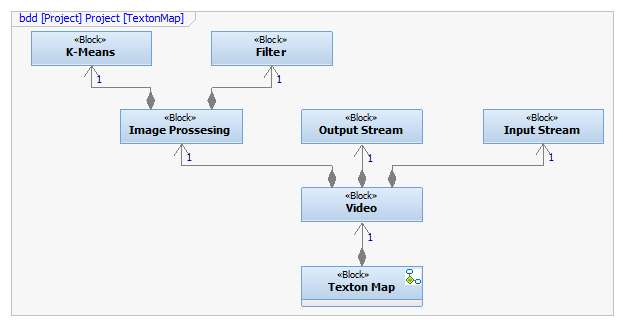
\includegraphics[width = 300 pt]{BlockDiagram}
\caption{Block diagram}
\label{fig:BlockDiagram}
\end{figure}

The top level block is called "Texton map", which is a block including the entire system. This block consists of three blocks; InputStream, ImageProcessing and OutputStream. The responsibility of the InputStream block is to read an image from a given camera and make it available for the ImageProcessing block. The OutputStream block is responsible for writing the output image to a given monitor. These two blocks are pure fictional and will not be a part of the SystemC model however they would be important in an actual system implementation. The ImageProcessing block consists of two sub blocks; Filtering and K-means according to section~\ref{sec:TextonFiltering}. In figure \ref{fig:InternalBlockDiagram} the internal block diagram of the ImageProcessing block is shown.

\begin{figure}[H]
\centering
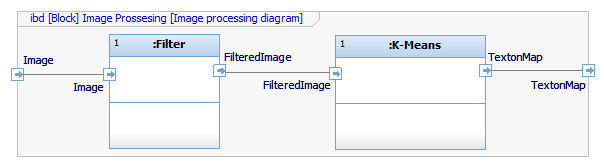
\includegraphics[width = 300 pt]{InternalBlockDiagram}
\caption{Internal Block diagram}
\label{fig:InternalBlockDiagram}
\end{figure}